\documentclass[11pt,a4paper]{article}
\usepackage[T1]{fontenc}
\usepackage{lmodern,microtype,amsmath,amsthm,amssymb,booktabs,array,graphicx,geometry,xcolor,hyperref}
\geometry{left=28mm,right=28mm,top=25mm,bottom=26mm}
\definecolor{ink}{HTML}{294B4A}
\hypersetup{colorlinks=true,linkcolor=ink,citecolor=ink,urlcolor=ink,
  pdftitle={Extremal laws for coupon collection with group drawings},pdfauthor={Anonymous}}
\newtheorem{theorem}{Theorem}[section]
\newtheorem{lemma}[theorem]{Lemma}
\newtheorem{corollary}[theorem]{Corollary}
\newtheorem{proposition}[theorem]{Proposition}
\theoremstyle{remark}
\newtheorem{remark}[theorem]{Remark}
\newtheorem{example}[theorem]{Example}
\newcommand{\E}{\mathbb E}
\newcommand{\ind}{\mathbf 1}
\setlength{\emergencystretch}{2em}
\title{Extremal laws for coupon collection with group drawings}
\author{Anonymous\\[3pt]{\small DOI \href{https://doi.org/10.5281/zenodo.24534721}{10.5281/zenodo.24534721}}}
\date{}
\begin{document}
\maketitle

\begin{abstract}
A collector repeatedly draws a random package of coupons and keeps every coupon it contains. How slowly, and how quickly, can a complete set be assembled? On the slow side we study \emph{fair} sampling laws, in which every coupon is equally likely to appear in a draw; Grunbaum and Yaakobi conjectured that drawing uniformly from all packages is the slowest fair law, and Barak-Pelleg and Berend disproved this with the Fano plane and asked how slow a fair law can be and how large the excess over uniform sampling can become. We show that when the omitted coupons can form the blocks of a Steiner $2$-design, sampling the complements of those blocks uniformly maximises the probability of being unfinished after every number of draws, and that this property characterises the design. For populations without designs we determine the asymptotic maximum mean in every critical window: if a draw omits a fraction $p$ of $n$ coupons and $np^k\to\lambda\in(0,\infty)$ for a fixed $k\ge2$, the slowest fair mean is $k+\min(1,\lambda)+o(1)$, compared with $k+1-e^{-\lambda}+o(1)$ for uniform sampling. We prove that for every $n$ and omitted size $r$ no fair law is slower than uniform sampling by more than $1/e+(1-\gamma)/\ln(n/r)$ draws on average, where $\gamma$ is Euler's constant, so the largest asymptotic excess when $r/n\to0$ is exactly $1/e$. An exhaustive exact search shows that the Fano plane attains the largest mean among all fair mechanisms at Barak-Pelleg and Berend's own parameters, and that six coupons in packages of three give the smallest counterexample to the Grunbaum--Yaakobi conjecture. On the fast side, a product inequality for independent Poisson clocks proves the conjecture of Fang and Chang: when the package size $s$ divides $n$, the mean is at least $(n/s)H_{n/s}$, with equality only for a uniform partition. A second bound, $1+n/s$, is sharp exactly when $n-s$ divides $n$.
\end{abstract}

\section{Introduction}
\label{sec:intro}
This section explains the problem, what was known, what this paper adds and how the paper is organised.

\paragraph{The problem.} In the classical coupon collector's problem a collector receives one uniformly random coupon out of $n$ types at each draw and needs on average $nH_n$ draws, where $H_n=1+\frac12+\cdots+\frac1n$, to see every type. In many settings each draw delivers a \emph{group} of coupons at once: a promotion puts several cards in each box, a sequencing run reads several fragments of a DNA library, a client contacts a subset of servers. The designer of the sampling law then controls how the groups overlap. Two natural questions are how to make complete collection as fast as possible, and how slow it can be made without unfair tricks such as making some coupons rare. Both questions have recently been posed explicitly, and this paper answers several of them.

\paragraph{What was known.} Fix $n$ coupons and a package size $s$ with $1\le s<n$. Call a sampling law \emph{fair} (or \emph{balanced}) if every coupon has the same probability $s/n$ of appearing in a draw. Grunbaum and Yaakobi \cite{gy} studied the fair mechanisms that sample uniformly from a family of distinct $s$-sets in which every coupon lies in the same number of sets, and conjectured \cite[Conjecture~2]{gy} that the \emph{full model}, sampling uniformly from all $\binom ns$ packages, is the slowest of them. Barak-Pelleg and Berend \cite{barak} disproved this: the seven lines of the Fano plane, used as packages of size three, are slower than the full model. They showed that their star mechanism is asymptotically slower than the full model in one regime and faster in another, and wrote that it remains open to determine the maximal possible expected coverage time among fair mechanisms and whether gaps substantially larger than theirs can occur.

On the fast side, Fang and Chang \cite{fang} proved that when $n=2s$ the uniform law on two complementary packages is the unique fastest law, and suggested that for every $s$ dividing $n$ the uniform law on a partition of the coupons into $n/s$ packages is optimal. Berend and Sher \cite{sher} record this as a conjecture of Fang and Chang; Fang and Chang report that the pairing case $s=2$ with $n$ even had been conjectured earlier in the operations-research literature, with $n=4$ and $n=6$ settled. Berend and Sher \cite{sher} proved Schilling's conjecture that the full model is not the fastest law for $2\le s\le n-2$, exhibiting faster partition-type laws, and Grunbaum and Yaakobi conjectured \cite[Conjecture~3]{gy} the lower bound $\lfloor n/s\rfloor H_{\lfloor n/s\rfloor}$ for their fair mechanisms.

\paragraph{What is new.} Table~\ref{tab:results} summarises the results. In brief:
\begin{itemize}
\item \emph{Slowest laws at finite size} (Section~\ref{sec:finite}). Among all fair laws, uniform sampling of the complements of the blocks of a Steiner $2$-design maximises $\Pr(T>j)$ for every $j$, and equality at any single $j\ge2$ forces the design. The same holds for partial coverage with higher designs.
\item \emph{Critical windows} (Section~\ref{sec:critical}). Write $r=n-s$ for the number of coupons a draw omits and $p=r/n$. For every population size, not just those carrying designs, the slowest fair mean is $k+\min(1,\lambda)+o(1)$ when $n\to\infty$ with $np^k\to\lambda\in(0,\infty)$ for a fixed $k\ge2$; here $np^k$ is the expected number of coupons still missing after $k$ draws. Barak-Pelleg and Berend's star mechanism already reaches $k+1$ in its own windows, where $\lambda>1$; the new content is the matching upper bound, attainment for every $\lambda$ including $\lambda<1$, and the exact peak excess $1/e$ at $\lambda=1$.
\item \emph{How much slower than the full model} (Section~\ref{sec:gap}). For all $n$ and $r=n-s$, every fair law has mean at most $1/e+(1-\gamma)/\ln(n/r)$ above the full model, where $\gamma=0.5772\ldots$ is Euler's constant. When packages hold at least half the coupons this is less than one draw, and as $r/n\to0$ the bound tends to $1/e$, which the critical windows attain.
\item \emph{Exact small cases} (Section~\ref{sec:small}). For $n\le7$, and for $n=8$ with $s\in\{2,6\}$, an exhaustive exact search finds the slowest fair mechanism. The full model is slowest except at $(n,s)=(6,3)$, $(7,3)$ and $(7,4)$. At $(7,3)$ the Fano plane attains the exact maximum, tied only with unions of two block-disjoint Fano planes.
\item \emph{Fastest laws} (Section~\ref{sec:minimum}). Every law on packages of size at most $s$ has $\E T\ge\max\{xH_x,\,1+x\}$ with $x=n/s$. This proves the Fang--Chang conjecture with uniqueness, and Grunbaum and Yaakobi's Conjecture~3 for all $n,s$. It also determines the minimum exactly when $n-s$ divides $n$.
\end{itemize}

\begin{table}[t]
\centering
\small
\begin{tabular}{@{}>{\raggedright\arraybackslash}p{3.3cm}>{\raggedright\arraybackslash}p{6.1cm}>{\raggedright\arraybackslash}p{3.6cm}@{}}
\toprule
Question & Answer here & Previously \\
\midrule
Slowest fair law, design parameters & Complements of Steiner $2$-design blocks, every horizon; characterisation (Thm~\ref{thm:steiner}) & Fano lines slower than full model \cite{barak} \\
Slowest fair mean, $np^k\to\lambda$ & $k+\min(1,\lambda)+o(1)$, any $n$ (Thm~\ref{thm:critical}) & Star mechanism reaches $k+1$ for its parameters, $\lambda>1$ \cite{barak} \\
Excess over the full model & $\le 1/e+(1-\gamma)/\ln(n/r)$ for all $n,r$; limit $1/e$ sharp (Thm~\ref{thm:gap}) & Asked in \cite{barak} \\
Small $n$ & Exact maxima for $n\le7$ (Prop.~\ref{prop:small}) & $(7,3)$ counterexample \cite{barak} \\
Fastest law, $s\mid n$ & $(n/s)H_{n/s}$, partitions only (Thm~\ref{thm:minimum}) & $n=2s$ \cite{fang}; conjectured \cite{fang,sher} \\
Fastest law, $(n-s)\mid n$ & $1+n/s$, omitted partitions only (Thm~\ref{thm:dualmin}) & Mean of this law computed \cite{sher} \\
\bottomrule
\end{tabular}
\caption{Summary of results. Here $n$ is the number of coupons, $s$ the package size, $r=n-s$ the number omitted per draw and $p=r/n$.}
\label{tab:results}
\end{table}

\paragraph{The main idea.} Every fair law has the same expected number of missing coupons after $j$ draws, namely $np^j$. What differs between laws is how the missing coupons cluster. A slow law makes them come in ones, so that the event ``something is missing'' is as likely as its expectation allows; designs and projective hyperplanes achieve this because their omitted blocks overlap in a controlled way. A fast law makes them come in large clumps that disappear together, which a partition into packages achieves. The slow side is controlled by the first two moments of the number of missing coupons, the fast side by a product inequality for independent Poisson clocks.

\paragraph{Related settings.} The probability that two independent draws of omitted sets meet is the intersection probability of a probabilistic quorum system \cite[Definition~3.1]{malkhi}, and the same clustering question arises when replicas are placed across machines that may fail. Falgas-Ravry, Larsson and Markstr\"om \cite{flm} study the concentration of the covering time for general random sets, using the same device of independent Poisson clocks attached to package types; they do not treat the extremal questions considered here.

\paragraph{Roadmap.} Section~\ref{sec:setting} fixes notation. Sections~\ref{sec:finite}--\ref{sec:small} treat slow collection: exact finite extremes, critical windows, the universal excess bound and exhaustive small cases. Section~\ref{sec:minimum} treats fast collection. Section~\ref{sec:open} lists open questions.

\section{Setting and notation}
\label{sec:setting}
This section fixes the notation used throughout.

Coupons are the points of $[n]=\{1,\dots,n\}$. A \emph{sampling law} is a probability distribution on subsets of $[n]$, called packages; draws are independent with this law. The \emph{collection time} $T$ is the first draw after which the union of the drawn packages is $[n]$, and $T\ge1$. For the slow side the packages have exactly $s$ coupons, $1\le s<n$; the complement of a package is its \emph{omitted set} $B$, of size $r=n-s$, and $p=r/n$. Write $B_1,B_2,\dots$ for the omitted sets of successive draws. After $j$ draws the coupons still missing form $\bigcap_{i\le j}B_i$, and we write
\[
 Z_j=\Big|\bigcap_{i=1}^j B_i\Big|,\qquad \Pr(T>j)=\Pr(Z_j>0)\quad(j\ge1),\qquad \E T=\sum_{j\ge0}\Pr(T>j).
\]
A law is \emph{balanced} (fair) if every coupon is omitted with probability $p$, equivalently appears with probability $s/n$. A \emph{regular family} is a family of distinct $s$-sets in which every coupon lies in the same number of members; the uniform law on a regular family is balanced, and these are the fair mechanisms of \cite{gy,barak}. A family of packages is regular exactly when the family of omitted sets is. The \emph{full model} is the uniform law on all $\binom ns$ packages; we write $T_{\rm full}$ for its collection time. A Steiner system $S(t,r,n)$ is a family of $r$-subsets of $[n]$, called blocks, such that every $t$-subset lies in exactly one block. For a $t$-$(n,r,\theta)$ design every $t$-subset lies in exactly $\theta$ blocks.

For the fast side we allow any law on packages of size \emph{at most} $s$. Write $\pi_A$ for the probability of package $A$ and $d_i=\sum_{A\ni i}\pi_A$ for the probability that coupon $i$ appears in one draw; then $\sum_i d_i=\E|A|\le s$. Put $x=n/s$ and extend the harmonic numbers to real $x>0$ by
\[
 H_x=\int_0^1\frac{1-(1-u)^x}{u}\,du ,
\]
which agrees with $\sum_{j\le x}1/j$ for integer $x$ and increases with $x$. Throughout, $\gamma=0.5772\ldots$ is Euler's constant.

\section{The slowest laws at finite size}
\label{sec:finite}
This section proves that complements of Steiner $2$-designs are the slowest fair laws whenever they exist, quantifies how close other laws can come, and extends the result to partial coverage.

\begin{theorem}[Slowest balanced collection]\label{thm:steiner}
Let $2\le r<n$ and $u=r(r-1)/(n(n-1))$. For every balanced law and every integer $j\ge1$,
\begin{equation}\label{eq:envelope}
 \Pr(T>j)\le n p^j-\frac{n(n-1)}{r}\,u^j .
\end{equation}
For any single $j\ge2$, equality holds if and only if the omitted set is uniform on the blocks of an $S(2,r,n)$. Such a law attains equality for every $j\ge1$, and its mean
\begin{equation}\label{eq:steinermean}
 1+\frac{np}{1-p}-\frac{n(n-1)}{r}\,\frac{u}{1-u}
\end{equation}
is the largest mean among balanced laws, hence also among fair mechanisms. A balanced law attains this mean only if it is uniform on the blocks of an $S(2,r,n)$.
\end{theorem}

\begin{proof}
For integers $0\le z\le r$,
\[
 \ind_{\{z>0\}}\le z-\frac2r\binom z2 ,
\]
because the difference is $0$ at $z=0$ and $(z-1)(r-z)/r\ge0$ for $1\le z\le r$, with equality exactly for $z\in\{0,1,r\}$. This is a degree-two polynomial bound of Bonferroni type; we claim no novelty for it. Apply it to $Z_j$. For a pair $\{a,b\}$ put $u_{ab}=\Pr(a,b\in B_1)$. Independence of the draws and balance give
\[
 \E Z_j=np^j,\qquad \E\binom{Z_j}{2}=\sum_{a<b}u_{ab}^{\,j},\qquad \sum_{a<b}u_{ab}=\binom r2,
\]
the last because each omitted set contains $\binom r2$ pairs. The average of the $u_{ab}$ is $u$, so convexity of $y\mapsto y^j$ gives $\sum_{a<b}u_{ab}^j\ge\binom n2u^j$, which proves \eqref{eq:envelope}.

Suppose equality holds at some $j\ge2$. Strict convexity forces $u_{ab}=u>0$ for every pair, and equality in the pointwise bound forces $Z_j\in\{0,1,r\}$ almost surely. If $B$ and $C$ are distinct omitted sets of positive probability, the sequence $B,C,B,\dots,B$ of $j$ draws has positive probability and leaves exactly $B\cap C$ missing, so $|B\cap C|\le1$. Since every pair has positive probability of being omitted, every pair lies in some supported block, and by the intersection bound in exactly one; the supported blocks therefore form an $S(2,r,n)$, and the mass of each block equals $u_{ab}=u$ for any pair inside it. Conversely, uniform sampling of an $S(2,r,n)$ gives every point the same omission probability (each point lies in the same number of blocks), every pair probability $u$, and $Z_j\in\{0,1,r\}$, so equality holds at every $j$.

Summing \eqref{eq:envelope} over $j\ge1$ and adding $\Pr(T>0)=1$ bounds $\E T$ by \eqref{eq:steinermean}, with equality for the design law. If a balanced law attains \eqref{eq:steinermean}, the nonnegative differences between the two sides of \eqref{eq:envelope} sum to zero, so equality holds at $j=2$ and the law is a design law. Uniform laws on regular families are balanced, and design laws are among them, which gives the statement about fair mechanisms.
\end{proof}

For $r=1$ balance determines the omission law, and for $r=2$ the design consists of all pairs. At $j=1$ both sides of \eqref{eq:envelope} equal one. When no $S(2,r,n)$ exists the bound is strict at every $j\ge2$; by compactness of the set of balanced laws the maximum of $\Pr(T>j)$ is then strictly smaller than \eqref{eq:envelope}, though the gap can be small. Explicit infinite families of Steiner $2$-designs, such as the lines of finite projective and affine spaces, give infinitely many parameter pairs to which the theorem applies.

\begin{proposition}[Two draws give an exact deficit]\label{prop:deficit}
Let $B,C$ be independent omitted sets with a common balanced law, $z=|B\cap C|$, and $U_2=np^2-n(n-1)u^2/r$. Then
\[
 U_2-\Pr(T>2)=\frac2r\sum_{a<b}(u_{ab}-u)^2+\frac1r\,\E\big[\ind_{\{z>0\}}(z-1)(r-z)\big].
\]
Consequently a balanced law whose two-draw deficit is at most $\epsilon$ has $\sum_{a<b}(u_{ab}-u)^2\le r\epsilon/2$ and, for $r>2$, intersections of intermediate size $2\le z\le r-1$ with probability at most $r\epsilon/(r-2)$.
\end{proposition}

\begin{proof}
Take expectations in $z-\frac2r\binom z2-\ind_{\{z>0\}}=\frac1r\ind_{\{z>0\}}(z-1)(r-z)$ and use $\sum_{a<b}u_{ab}^2-\binom n2u^2=\sum_{a<b}(u_{ab}-u)^2$, which holds because the $u_{ab}$ have mean $u$. For the last claim, $(z-1)(r-z)\ge r-2$ when $2\le z\le r-1$.
\end{proof}

\begin{example}[Seven coupons]\label{ex:seven}
On $\mathbb Z/7\mathbb Z$ the seven translates of $\{0,1,3\}$ contain every pair exactly once, because the six differences of $\{0,1,3\}$ exhaust the nonzero residues; they are the lines of the Fano plane. Omit one of these lines uniformly and collect its four-point complement. Any two lines meet, so collection in two draws is impossible, whereas uniform four-coupon draws finish at the second draw with probability $4/35$. Both laws omit each point with probability $3/7$ and each pair with probability $1/7$. Inclusion--exclusion gives
\[
 \Pr(T_{\rm design}>j)-\Pr(T_{\rm full}>j)=7^{1-j}-35^{1-j}\qquad(j\ge1),
\]
and the means are $47/12$ for the design and $257/68$ for the full model, an excess of $7/51$. By Theorem~\ref{thm:steiner} this design law is the exact slowest fair law for $n=7$ and $s=4$. Barak-Pelleg and Berend's Fano example \cite{barak} uses the seven lines themselves as packages of size three, a different parameter pair; Section~\ref{sec:small} shows that it is the exact maximum there too.
\end{example}

\subsection*{Partial coverage and higher designs}
For $1\le h<r$ let $S_h$ be the first draw after which fewer than $h$ coupons remain missing, so $S_1=T$. Set $p_d=\binom rd/\binom nd$. The next theorem assumes that every $h$-subset is omitted with the same probability $p_h$; for $h>1$ this is stronger than balance, and it holds for designs of strength $h$.

\begin{theorem}[Partial coverage]\label{thm:higher}
With $c=(\binom rh-1)/\binom r{h+1}$,
\[
 \Pr(S_h>j)\le \binom nh p_h^j-c\binom n{h+1}p_{h+1}^j,\qquad j\ge1 .
\]
Under the hypothesis above, equality at any $j\ge2$ holds if and only if the omitted set is uniform on the blocks of an $S(h+1,r,n)$, which attains equality at every $j$.
\end{theorem}
\begin{proof}
Let $f(z)=\binom zh-c\binom z{h+1}$, with binomial coefficients vanishing when the lower index exceeds the upper. Then $f(z)=0$ for $z<h$, $f(h)=1$ and $f(r)=\binom rh-(\binom rh-1)=1$. We show $f(z)>1$ for $h<z<r$. The first difference $\Delta f(z)=f(z+1)-f(z)=\binom z{h-1}-c\binom zh$ changes sign at most once, from positive to negative, because $\binom z{h-1}/\binom zh=h/(z-h+1)$ strictly decreases. If $r=h+1$ there is nothing to prove. Otherwise $\Delta f(h)>0$: if $\Delta f(h)\le0$, then $\Delta f(z)<0$ for all $z>h$ and $f(r)<f(h)$, a contradiction. Hence $f$ rises strictly from $f(h)=1$, then falls, with at most one zero difference at the turn, to $f(r)=1$, so every intermediate value exceeds one. Therefore $\ind_{\{z\ge h\}}\le f(z)$ on $0\le z\le r$, with equality exactly for $z\le h$ and $z=r$.

Since $S_h>j$ exactly when $Z_j\ge h$, take expectations in $\ind_{\{Z_j\ge h\}}\le f(Z_j)$. The hypothesis gives $\E\binom{Z_j}h=\binom nhp_h^j$. The average over $(h+1)$-sets of their omission probabilities is $p_{h+1}$, so convexity gives $\E\binom{Z_j}{h+1}\ge\binom n{h+1}p_{h+1}^j$. For equality at some $j\ge2$ all $(h+1)$-sets must have the same positive omission probability and $Z_j\in\{0,\dots,h\}\cup\{r\}$ almost surely; as in Theorem~\ref{thm:steiner}, distinct supported blocks meet in at most $h$ points, so each $(h+1)$-set lies in exactly one block, which determines its mass. Conversely an $S(h+1,r,n)$ has every $h$-set in the same number of blocks, distinct blocks meeting in at most $h$ points, and gives equality.
\end{proof}

\section{The slowest fair collector at a critical scale}
\label{sec:critical}
This section determines the largest mean over fair laws, to within $o(1)$, along every sequence of parameters at which the full model has a nondegenerate chance of being unfinished after a fixed number of draws.

Fix an integer $k\ge2$ and let $n\to\infty$ with omitted size $r=r(n)$ and $p=r/n$ such that $np^k\to\lambda\in(0,\infty)$. Then $p=(\lambda/n)^{1/k}(1+o(1))\to0$ and $r=np\to\infty$. At this scale the full model is unfinished after $k$ draws with probability tending to $1-e^{-\lambda}$, and its mean tends to $k+1-e^{-\lambda}$ \cite{berend-asym}.

\begin{theorem}\label{thm:critical}
In this regime, the maximum of $\E T$ over balanced laws on $r$-subsets, and also over fair mechanisms (uniform laws on regular families), satisfies
\[
  \max \E T = k+\min\{1,\lambda\}+o(1).
\]
In each class there are laws with $\Pr(T=k+1)\to\min\{1,\lambda\}$ and $\Pr(T=k)\to1-\min\{1,\lambda\}$. The full model has $\E T_{\rm full}=k+1-e^{-\lambda}+o(1)$, so the asymptotic excess of the slowest fair law over the full model is $\min\{1,\lambda\}-1+e^{-\lambda}$. It is largest, equal to $e^{-1}$, at $\lambda=1$.
\end{theorem}

\begin{figure}[htb]
\centering
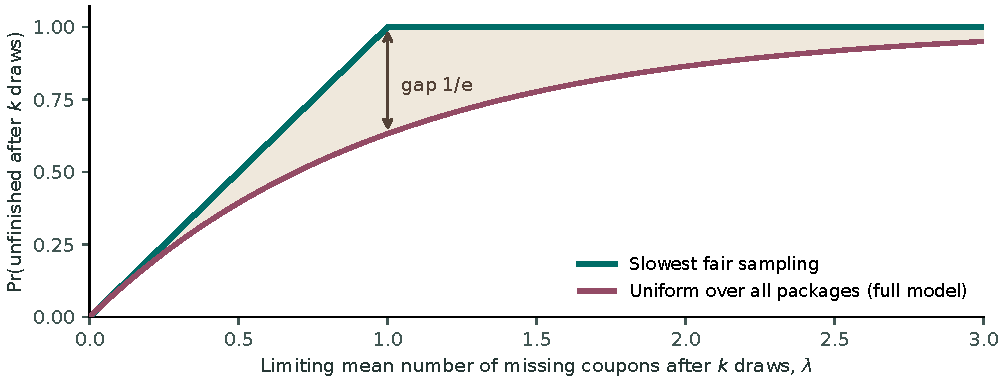
\includegraphics[width=.91\linewidth]{figures/critical-window.pdf}
\caption{Limiting probability of being unfinished after $k$ draws, as a function of $\lambda=\lim np^k$. Every fair law has the same expected number of missing coupons, $np^k$; the slowest law makes them appear one at a time (upper curve), while the full model lets them form a Poisson number (lower curve). The vertical distance is also the limiting difference of the mean collection times; it peaks at $1/e$ when $\lambda=1$.}
\label{fig:gap}
\end{figure}

\begin{remark}[The star mechanism]\label{rem:star}
Barak-Pelleg and Berend's star mechanism \cite[Theorem~2.4]{barak} lies in these windows. For fixed $c\ge2$ its coupons are the $(m-c)$-subsets of $[m]$, so $n=\binom mc$, and each draw picks a uniform centre $i\in[m]$ and reveals every coupon containing $i$. A coupon is omitted by a draw exactly when it avoids the centre, so $p=c/m$ and $np^c\to\beta_c=c^c/c!\ge2$: the mechanism lies in the window with $k=c$ and $\lambda=\beta_c$. A coupon avoids a set of centres unless that set has at least $c+1$ elements, so collection needs $c+1$ distinct centres and $T\ge c+1$ always. It therefore attains the maximum $k+1$ of Theorem~\ref{thm:critical}, and its excess $e^{-\beta_c}$ over the full model agrees with $\min\{1,\lambda\}-1+e^{-\lambda}$ at $\lambda=\beta_c$. What is new here is the matching upper bound, attainment for every $\lambda$ and every population size, including $\lambda<1$ where the maximum $k+\lambda$ requires thinning, and the peak excess $1/e$.
\end{remark}

\begin{proof}[Proof of Theorem~\ref{thm:critical}]
\emph{Upper bound.} Write $X_j=Z_j$ for the number of coupons missing after $j$ draws. Every balanced law has $\E X_j=np^j$, so $\Pr(T>j)\le\min\{1,np^j\}$ for $j\ge1$. (The same first-moment estimate underlies \cite[Theorem~10]{gy}.) Split $\E T=\sum_{j\ge0}\Pr(T>j)$ into the terms $0\le j<k$, which contribute at most $k$; the term $j=k$, at most $\min\{1,np^k\}\to\min\{1,\lambda\}$; and the terms $j>k$, at most $\sum_{j>k}np^j=np^{k+1}/(1-p)=o(1)$. This gives $\E T\le k+\min\{1,\lambda\}+o(1)$.

\emph{Construction.} Let $q$ be the largest prime with $N=1+q+\cdots+q^k\le n$. By the prime number theorem consecutive primes have ratio tending to one, so $q\sim n^{1/k}$ and $N/n\to1$. Identify $N$ of the coupons, the \emph{core}, with the points of the projective space $\mathrm{PG}(k,q)$, the one-dimensional subspaces of $\mathbb F_q^{k+1}$; a hyperplane contains $h=1+q+\cdots+q^{k-1}$ points. Independently at each draw, choose a uniformly random hyperplane $H$, and choose an integer $d\in\{\lfloor Np\rfloor,\lceil Np\rceil\}$ with mean $Np$. If $d\le h$, put a uniformly random $d$-subset of $H$ into the omitted set; if $d>h$, put all of $H$ and $d-h$ uniformly random core points outside $H$. Finally add $r-d$ uniformly random points outside the core. This is feasible: since $r$ is an integer, $r-d$ takes the values $\lceil(n-N)p\rceil$ and $\lfloor(n-N)p\rfloor$, which lie in $[0,n-N]$, and when $N=n$ the last step is empty. The law is invariant under the collineation group, which is transitive on core points, so every core point is omitted with probability $\E d/N=p$; points outside the core are omitted with probability $\E(r-d)/(n-N)=p$. So the law is balanced.

Given $H$ and $d$, each point of $H$ is omitted with probability $\alpha_d=\min\{1,d/h\}$. Since $Np/h\sim qp\to\lambda^{1/k}$, we have $\alpha_d\to a=\min\{1,\lambda^{1/k}\}$ uniformly over the two values of $d$.

\emph{Horizon $k$.} Any $k$ hyperplanes of $\mathrm{PG}(k,q)$ share at least one point, because $k$ hyperplanes of $\mathbb F_q^{k+1}$ intersect in a subspace of dimension at least one. Conditional on the hyperplanes and sizes of $k$ draws, fix one common point by a fixed ordering of the core; it is omitted by all $k$ draws with probability $\prod_{i\le k}\alpha_{d_i}$. Hence $\Pr(T>k)\ge\E\prod_i\alpha_{d_i}\to a^k=\min\{1,\lambda\}$, and with the upper bound $\Pr(T>k)\to\min\{1,\lambda\}$.

\emph{Horizons $j<k$.} Any $j$ hyperplanes share a subspace of dimension at least $k+1-j\ge2$, hence at least $q+1$ projective points. Conditional on the hyperplanes and sizes, let $W$ count the common points omitted at all $j$ draws. Within one draw the omission indicators of two points of $H$ have nonpositive covariance (uniform sampling without replacement, or retaining all of $H$), and since draws are independent the probability that two points survive all $j$ draws is at most the product of their survival probabilities. Hence $\mathrm{Var}\,W\le\E W$, and $\E W\ge(q+1)(a/2)^j$ for large $n$. Chebyshev's inequality gives $\Pr(W=0)\le1/\E W\to0$, so $\Pr(T>j)\to1$.

The tail estimate from the upper bound gives $\Pr(T>k+1)\le np^{k+1}=o(1)$. Combining, $\Pr(T=k+1)\to\min\{1,\lambda\}$, $\Pr(T=k)\to1-\min\{1,\lambda\}$ and $\E T=k+\min\{1,\lambda\}+o(1)$ for this balanced law. Lemma~\ref{lem:regularisation} below, applied with $K=k$, replaces it by a fair mechanism whose probabilities $\Pr(T>j)$ change by $o(1)$ for $2\le j\le k$; the term $j=1$ is always one and the terms $j>k$ remain $o(1)$, so the same limits hold for fair mechanisms.

\emph{Full model.} For uniform omitted $r$-sets the factorial moments of $X_j$ are $\E(X_j)_a=(n)_a\big((r)_a/(n)_a\big)^j$, where $(y)_a=y(y-1)\cdots(y-a+1)$. For fixed $a$ and $j=k$ they converge to $\lambda^a$, since $r\to\infty$, so $X_k$ converges in law to a Poisson($\lambda$) variable and $\Pr(T_{\rm full}>k)\to1-e^{-\lambda}$, in agreement with \cite{berend-asym}. For $j<k$ two coupons are jointly omitted with probability at most the product of their omission probabilities and $np^j\to\infty$, so $\Pr(X_j>0)\to1$ by Chebyshev's inequality. The tail estimate gives $\E T_{\rm full}=k+1-e^{-\lambda}+o(1)$. Finally $g(\lambda)=\min\{1,\lambda\}-1+e^{-\lambda}$ has derivative $1-e^{-\lambda}>0$ on $(0,1)$ and $-e^{-\lambda}<0$ on $(1,\infty)$, so its maximum is $g(1)=e^{-1}$.
\end{proof}

The theorem is asymptotic and the convergence is slow. For example, with $k=2$ and $r=\sqrt n$ (so $np^2=1$) the exact full-model mean is $2.7769$ at $n=100$, $2.7022$ at $n=400$ and $2.6667$ at $n=1600$, against the limit $3-e^{-1}=2.6321$. The excess $1/e$ is a limiting value, not a finite-$n$ guarantee.

The following lemma transfers a balanced law to a fair mechanism. Its constants are chosen only to leave slack in two union bounds.

\begin{lemma}[Regularisation]\label{lem:regularisation}
Suppose $r\to\infty$ and $p=r/n\to0$. Given a balanced law on $r$-subsets of $[n]$ and a fixed integer $K\ge2$, there is a uniform law on a regular family of distinct $r$-subsets such that, for every $2\le j\le K$, the probabilities that $j$ independent draws have a common point differ by $o(1)$ as $n\to\infty$.
\end{lemma}

\begin{proof}
\emph{Smoothing.} For large $n$, modify each drawn set $B$ by exchanging $D=25$ uniformly chosen elements of $B$ with $D$ uniformly chosen elements outside $B$. The new law $\nu$ is balanced: a point is omitted with probability $p(1-D/r)+(1-p)D/(n-r)=p-D/n+D/n=p$. Every transition probability to a specified set is zero or $[\binom rD\binom{n-r}D]^{-1}$, so every atom of $\nu$ is at most this value. Replacing one draw by its smoothed version changes the event ``all $j$ draws share a point'' only if one of the $2D$ exchanged elements lies in all the other $j-1$ draws; those draws are independent of it and balanced, so this has probability at most $2Dp^{j-1}$. Replacing the $j$ draws one at a time changes the probability by at most $2jDp^{j-1}=o(1)$.

\emph{Sampling.} Draw $M=n^8$ independent rows from $\nu$. With probability tending to one, four properties hold.
(i) Distinct rows are at Johnson distance at least three, where the distance between $r$-sets is the number of single exchanges needed to pass from one to the other. A ball of radius two contains $1+r(n-r)+\binom r2\binom{n-r}2=O(n^4)$ sets, so by the atom bound and a union bound over pairs the failure probability is $O(M^2n^4)/[\binom rD\binom{n-r}D]=O(n^{20}/n^{25})=o(1)$.
(ii) Every point lies in $Mp+O(\sqrt{M\log n})$ rows, by Hoeffding's inequality and a union bound over points.
(iii) For every ordered pair of distinct points $u,v$, at least $cM/n$ rows contain $u$ and omit $v$, for an absolute constant $c>0$. Indeed both points are absent from the original set with probability at least $1-2p$, and then the added elements include $u$ but not $v$ with probability $D(n-r-D)/[(n-r)(n-r-1)]$, which is at least a constant times $1/n$; a binomial lower-tail bound and a union bound over pairs finish the claim.
(iv) For $2\le j\le K$ the empirical law of the rows gives the common-point probabilities within $o(1)$ of those of $\nu$. Choosing $j$ row indices independently and uniformly, an index repeats with probability $O_K(1/M)$, and on distinct indices the rows have law $\nu^{\otimes j}$; so the expected empirical probability is within $O_K(1/M)$ of the $\nu$ value. Changing one row moves the empirical probability by at most $j/M$, and the bounded differences inequality gives concentration at the finitely many horizons.

\emph{Repair.} Fix a sample with (i)--(iv). The target degree $Mp=n^7r$ is an integer and the degrees sum to $Mr$. While some degree differs from the target, choose a point $u$ above target and a point $v$ below it, and in one not yet modified row containing $u$ and omitting $v$ replace $u$ by $v$. Each exchange reduces the total absolute deviation by two, so at most $O(n\sqrt{M\log n})=O(n^5\sqrt{\log n})=o(M/n)$ exchanges are needed, and by (iii) an unmodified witness row is always available. Each row is modified at most once, so it moves Johnson distance at most one, and (i) keeps the final rows distinct. The final rows form a regular family of distinct $r$-sets. The uniform law on them differs from the empirical law in total variation by the fraction of modified rows, which is $o(1)$, and $j$ independent draws multiply this by at most $j$.
\end{proof}

\section{How much slower than the full model can a fair law be?}
\label{sec:gap}
This section addresses the second question of Barak-Pelleg and Berend, how large the excess over the full model can be. For every population size the excess of any fair law is bounded by an explicit quantity, which tends to $1/e$ when the omitted fraction tends to zero; in that limit the bound is sharp. The proof combines the first-moment upper bound for fair laws with a lower bound for the full model obtained from negative dependence.

\begin{lemma}[Hypergeometric generating function]\label{lem:pgf}
Let $B$ be a uniformly random $r$-subset of $[n]$, $p=r/n$, and $S\subseteq[n]$ with $|S|=w$. For $0\le y\le1$,
\[
 \E\, y^{|B\cap S|}\le(1-p+py)^w .
\]
\end{lemma}
\begin{proof}
Induct on $w$; the case $w=0$ is trivial. Pick $b\in S$, let $S'=S\setminus\{b\}$ and $\xi=\ind_{\{b\in B\}}$, and put $g(\xi)=\E[y^{|B\cap S'|}\mid\xi]$. Given $\xi=1$, $B\setminus\{b\}$ is a uniform $(r-1)$-subset of $[n]\setminus\{b\}$; given $\xi=0$, $B$ is a uniform $r$-subset of $[n]\setminus\{b\}$. Deleting a uniformly chosen element of the latter produces the former, so $|B\cap S'|$ is stochastically smaller given $\xi=1$, and since $y^m$ decreases in $m$, $g(1)\ge g(0)$. The function $\phi(\xi)=y^\xi$ is nonincreasing, so $\mathrm{Cov}(\phi(\xi),g(\xi))=\Pr(\xi=1)\Pr(\xi=0)(\phi(1)-\phi(0))(g(1)-g(0))\le0$. Hence $\E y^{|B\cap S|}=\E[\phi(\xi)g(\xi)]\le\E\phi(\xi)\,\E g(\xi)=(1-p+py)\,\E y^{|B\cap S'|}$, and the induction hypothesis finishes the proof.
\end{proof}

\begin{proposition}[Full-model tails]\label{prop:fulltail}
For the full model and every $j\ge1$,
\[
 \Pr(T_{\rm full}>j)\ge1-(1-p^j)^n\ge1-e^{-np^j}.
\]
\end{proposition}
\begin{proof}
Let $I_m=\bigcap_{i\le m}B_i$, with $I_0=[n]$. Given $I_{j-1}$, collection is complete after draw $j$ exactly when $B_j\cap I_{j-1}=\emptyset$; Lemma~\ref{lem:pgf} with $y=0$ bounds the conditional probability by $(1-p)^{|I_{j-1}|}$, so $\Pr(T_{\rm full}\le j)\le\E y_1^{|I_{j-1}|}$ with $y_m=1-p^m$. For any $i\ge1$ and $m\ge1$, Lemma~\ref{lem:pgf} applied to $|I_i|=|B_i\cap I_{i-1}|$ gives $\E[y_m^{|I_i|}\mid I_{i-1}]\le(1-p+py_m)^{|I_{i-1}|}=y_{m+1}^{|I_{i-1}|}$. Applying this successively with $(i,m)=(j-1,1),(j-2,2),\dots,(1,j-1)$ gives $\E y_1^{|I_{j-1}|}\le\E y_2^{|I_{j-2}|}\le\cdots\le y_j^{|I_0|}=(1-p^j)^n$. The second inequality is $1-y\le e^{-y}$.
\end{proof}

\begin{lemma}[Sums over a geometric grid]\label{lem:grid}
Let $\phi:\mathbb R\to[0,\infty)$ be nondecreasing on $(-\infty,x^*]$ and nonincreasing on $[x^*,\infty)$, and let the points $x_1>x_2>\cdots$ be spaced $\Delta>0$ apart. Then $\sum_i\phi(x_i)\le\sup\phi+\Delta^{-1}\int_{\mathbb R}\phi$.
\end{lemma}
\begin{proof}
Let $L$ be the largest grid point below $x^*$ and $R=L+\Delta$ (if either does not exist the argument simplifies). Each grid point $x<L$ satisfies $\phi(x)\le\Delta^{-1}\int_x^{x+\Delta}\phi$ by monotonicity, and each grid point $x>R$ satisfies $\phi(x)\le\Delta^{-1}\int_{x-\Delta}^{x}\phi$. On $[L,R]$, $\phi\ge\min\{\phi(L),\phi(R)\}$, so $\phi(L)+\phi(R)\le\sup\phi+\Delta^{-1}\int_L^R\phi$. The intervals used are disjoint.
\end{proof}

\begin{theorem}[Universal excess bound]\label{thm:gap}
Let $1\le r<n$ and $p=r/n$. For every balanced law on $r$-subsets,
\[
 \E T-\E T_{\rm full}\ \le\ \sum_{j\ge1}\Big[\min\{1,np^j\}-1+(1-p^j)^n\Big]\ \le\ \frac1e+\frac{1-\gamma}{\ln(n/r)} .
\]
In particular the excess is below one draw whenever $r\le n/2$ (the bound is then at most $0.978$), and as $r/n\to0$ the largest excess of a fair law over the full model is at most $1/e+o(1)$. This limit is attained: in the window $k=2$, $\lambda=1$ of Theorem~\ref{thm:critical} the largest excess tends to $1/e$.
\end{theorem}
\begin{proof}
The first inequality combines $\Pr(T>j)\le\min\{1,np^j\}$ for balanced laws with Proposition~\ref{prop:fulltail}; the terms $j=0$ cancel. Each summand is at most $h(np^j)$, where $h(\mu)=\min\{1,\mu\}-1+e^{-\mu}\ge0$. On the logarithmic scale $\phi(t)=h(e^t)$ is increasing for $t<0$ and decreasing for $t>0$, with maximum $h(1)=e^{-1}$, and the points $t_j=\ln(np^j)$ are spaced $\Delta=\ln(1/p)=\ln(n/r)$ apart. Lemma~\ref{lem:grid} bounds the sum by $e^{-1}+\Delta^{-1}\int_0^\infty h(\mu)\,d\mu/\mu$. Finally
\[
 \int_0^\infty\frac{h(\mu)}{\mu}\,d\mu=\int_0^1\Big(1-\frac{1-e^{-\mu}}{\mu}\Big)d\mu+\int_1^\infty\frac{e^{-\mu}}{\mu}\,d\mu=1-\mathrm{Ein}(1)+E_1(1)=1-\gamma,
\]
using $\mathrm{Ein}(1)=\int_0^1(1-e^{-\mu})\mu^{-1}d\mu$, $E_1(1)=\int_1^\infty e^{-\mu}\mu^{-1}d\mu$ and the identity $\mathrm{Ein}(z)=E_1(z)+\gamma+\ln z$ at $z=1$. At $r=n/2$ the bound is $e^{-1}+(1-\gamma)/\ln2=0.9778\ldots$. The attainment statement is Theorem~\ref{thm:critical} with $\lambda=1$.
\end{proof}

The bound is uniform over all parameters and also covers Barak-Pelleg and Berend's star mechanism, whose excess $e^{-\beta_c}$ is below $1/e$. For small packages, with $r/n\to1$, it grows like $(1-\gamma)n/s$; whether the excess of fair laws over the full model can actually grow without bound is open (Section~\ref{sec:open}).

\section{Exact maxima for small populations}
\label{sec:small}
This section reports an exhaustive computation of the slowest fair mechanism for all small parameter pairs, which answers Barak-Pelleg and Berend's question exactly at their own example.

\begin{proposition}[Computer-assisted]\label{prop:small}
For $n\le7$ and all $1\le s<n$, and for $n=8$ with $s\in\{2,6\}$, the slowest fair mechanism is the full model, uniquely, except in the three cases of Table~\ref{tab:small}. The cases $s=1$ and $s=n-1$ are trivial, since balance then leaves only the full model. In particular the Fano plane, with its lines as packages, attains the largest mean among fair mechanisms for seven coupons in packages of three (tied only with the unions of two block-disjoint Fano planes), and six coupons in packages of three give the smallest counterexample to the conjecture that the full model is the slowest fair mechanism \cite[Conjecture~2]{gy}.
\end{proposition}

\begin{table}[ht]
\centering
\small
\begin{tabular}{@{}ccrlll@{}}
\toprule
$n$ & $s$ & fair mechanisms & slowest mean & full model & slowest families \\
\midrule
6 & 3 & 3{,}435 & $157/36\approx4.3611$ & $4.3026$ & the $2$-$(6,3,2)$ design (12 labelled copies) \\
7 & 3 & 2{,}505{,}121 & $163/30\approx5.4333$ & $5.4201$ & 30 Fano planes; 120 unions of two \\
 & & & & & \quad block-disjoint Fano planes \\
7 & 4 & 2{,}505{,}121 & $47/12\approx3.9167$ & $3.7794$ & 30 complements of Fano planes \\
\bottomrule
\end{tabular}
\caption{The parameter pairs with $n\le7$ at which the full model is not the slowest fair mechanism. Packages have size $s$. The exact full-model means are $327/76$, $85691/15810$ and $257/68$, so the exact excesses are $10/171$, $7/527$ and $7/51$.}
\label{tab:small}
\end{table}

\emph{Method.} For each $(n,s)$ the program \nolinkurl{code/fair_maxima.c} enumerates every family of distinct $s$-subsets of $[n]$ with equal point degrees and computes $\E T$ by the exact recursion over covered sets, $\E[S]=\big(|\mathcal F|+\sum_{A:\,S\cup A\ne S}\E[S\cup A]\big)/|\{A:S\cup A\ne S\}|$, in double precision. Each value is obtained by at most $n$ levels of the recursion, each forming a sum of at most $\binom ns+1\le71$ positive terms and one division, so its relative rounding error is at most about $75n$ units in the last place, below $10^{-12}$, while the largest and second largest distinct values differ by more than $10^{-6}$ in every case. The script \nolinkurl{code/certify_fair_maxima.py} checks this separation, recomputes every maximiser and the full model in exact rational arithmetic, and verifies the stated structure of the maximisers. In all three exceptional cases the omitted sets of the maximisers have equal pair-omission probabilities, the property singled out by Theorem~\ref{thm:steiner}.

\section{The fastest sampling laws}
\label{sec:minimum}
This section proves two lower bounds on the mean collection time for arbitrary laws on packages of size at most $s$, each sharp for a divisibility family, and identifies all minimisers in those families.

\begin{lemma}[Product bound for independent coordinates]\label{lem:read}
Let $Y_1,\dots,Y_n$ be nonnegative functions of independent coordinates, and suppose each coordinate enters at most $s$ of these functions. Then
\[
 \E\prod_{i=1}^nY_i\le\prod_{i=1}^n(\E Y_i^s)^{1/s}.
\]
\end{lemma}
\begin{proof}
Integrate out one coordinate with the others fixed. H\"older's inequality with $s$ equal exponents bounds the integral of the product of the affected functions by the product of their conditional $L^s$ norms (padding with factors equal to one if fewer than $s$ functions are affected). Iterate over the remaining coordinates; for each function the successive $s$th powers and roots telescope. This is the case $p_j=s$ of Finner's generalized H\"older inequality \cite[Theorem~2.1 and (3.1)]{finner}: there the $j$th function has exponent $p_j$ and $M_i$ is the set of functions depending on coordinate $i$, and for probability measures Finner notes that the condition $\sum_{j\in M_i}p_j^{-1}=1$ may be weakened to $\le1$; and here each coordinate lies in at most $s$ of the index sets, so the sum is at most $s\cdot s^{-1}=1$. Pelekis, Ramon and Wang restate the inequality as \cite[Theorem~2.1]{pelekis}.
\end{proof}

Attach to the draws the arrival times of a rate-one Poisson process, and mark each arrival independently with a package drawn from the law $\pi$. The numbers $N_A(t)$ of arrivals carrying package $A$ by time $t$ are then independent Poisson variables with means $t\pi_A$; the same device is used in \cite{flm}. For an integer $h\ge1$ let $T_h$ be the number of draws until every coupon has appeared at least $h$ times, so $T_1=T$, and let $\tau_h$ be the corresponding arrival time. Given $T_h=m$, $\tau_h$ is a sum of $m$ independent mean-one exponential variables, because the marks alone determine $T_h$; hence $\E\tau_h=\E T_h$.

\begin{theorem}[Poisson-time comparison]\label{thm:poisson}
Let $G_h(z)=\Pr\{\mathrm{Poisson}(z)\ge h\}$. For every law on packages of size at most $s$ and every $t>0$,
\begin{equation}\label{eq:read-min}
 \Pr\{\tau_h\le t\}\le\prod_{i=1}^nG_h(td_i)^{1/s}\le G_h(t/x)^x .
\end{equation}
If $s\mid n$, the uniform law on the blocks of a partition of $[n]$ into $s$-sets attains equality for every $t$ and $h$, and for each fixed $h$ it is the unique minimiser of $\E T_h$ up to relabelling.
\end{theorem}
\begin{proof}
Apply Lemma~\ref{lem:read} to the indicators that each coupon has reached its quota $h$ by time $t$. The indicator for coupon $i$ depends only on the counts $N_A(t)$ with $A\ni i$, so each count enters at most $s$ indicators; the count of arrivals containing $i$ is Poisson with mean $td_i$. This gives the first inequality. For $h=1$ this is the avoidance bound of Pelekis, Ramon and Wang \cite[Theorem~2.6]{pelekis} applied to the Poisson counts.

For the second inequality, $\log G_h$ is strictly increasing and strictly concave on $(0,\infty)$: with $G_h(0)=0$ and $G_h'(z)=e^{-z}z^{h-1}/(h-1)!$ one has $G_h(z)/G_h'(z)=\int_0^z(1-v/z)^{h-1}e^v\,dv$, which strictly increases, so the logarithmic derivative strictly decreases. Jensen's inequality and $\sum_id_i\le s$ give $\frac1s\sum_i\log G_h(td_i)\le\frac ns\log G_h(t/x)$. If some $d_i=0$ the left side of \eqref{eq:read-min} vanishes; otherwise equality in the second inequality at any $t>0$ forces $d_i=s/n$ for all $i$. For the uniform partition all coupons of one block have the same count, and the $x$ block counts are independent Poisson variables with mean $t/x$, which gives equality.

It remains to show that a law with $\Pr\{\tau_h\le t\}=G_h(t/x)^x$ for every $t$ is a uniform partition; this suffices for the means, because the difference between the two sides of \eqref{eq:read-min} is continuous and nonnegative, so equal means force equality for all $t$. All rates equal $d=1/x$. Group coupons into classes according to the set of positive-probability packages containing them; two coupons in one class always have equal counts. For coupons in different classes, the total rate $d'$ of packages containing at least one of them exceeds $d$. If both fall short of $h$, the arrivals of these package types number at most $2h-2$, which has probability $O\big((1+t^{2h-2})e^{-d't}\big)$, while a single class falls short with probability $1-G_h(dt)\sim e^{-dt}(dt)^{h-1}/(h-1)!$. Taking one representative from each of the $K$ classes, the first two Bonferroni inequalities give $\Pr\{\tau_h>t\}\sim K[1-G_h(dt)]$ as $t\to\infty$. The extremal tail is $1-G_h(dt)^x\sim x[1-G_h(dt)]$, so $K=x$. Each class lies inside a positive-probability package, so it has at most $s$ coupons, and $K=x$ classes cover $n=xs$ coupons; hence every class has exactly $s$ coupons, every supported package is one class (packages have at most $s$ coupons and are unions of classes, and empty packages are excluded because $\sum_id_i=s$), and each has probability $d$.
\end{proof}

\begin{theorem}[Minimum expected collection time]\label{thm:minimum}
Every law on packages of size at most $s$ satisfies $\E T\ge xH_x$ with $x=n/s$. Equality holds exactly when $s$ divides $n$ and the law is uniform on the blocks of a partition of $[n]$ into $s$-sets.
\end{theorem}
\begin{proof}
Take $h=1$ in \eqref{eq:read-min}, integrate the survival function and substitute $u=e^{-t/x}$:
\[
 \E T=\E\tau_1\ge\int_0^\infty\big[1-(1-e^{-t/x})^x\big]dt=x\int_0^1\frac{1-(1-u)^x}{u}\,du=xH_x .
\]
Equality forces $K=x$ in the proof of Theorem~\ref{thm:poisson}, so $x$ is an integer and the law is a uniform partition, which attains equality.
\end{proof}

For $s\mid n$ this proves the conjecture recorded by Fang and Chang \cite{fang} and Berend and Sher \cite{sher}, including uniqueness; for $s=2$ it covers the pairing case for every even $n$. Since $xH_x$ increases with $x$, it is at least $\lfloor x\rfloor H_{\lfloor x\rfloor}$, which proves Grunbaum and Yaakobi's Conjecture~3 \cite{gy} for all $n$ and $s$, and for all laws rather than only fair mechanisms. Grunbaum and Yaakobi remark that the divisible lower bound had been stated to extend from the case $n=2s$ \cite[Remark~2 and Section~VII]{gy}, attributing this to Berend and Sher; both arXiv versions of Berend and Sher's paper \cite{sher} treat general divisibility as a conjecture of Fang and Chang, and we are not aware of an earlier complete proof. For $s\mid n$, \eqref{eq:read-min} also gives $\E z^{T_h}\le\E z^{T_h^*}$ for $0<z<1$, where $T_h^*$ is the draw count of the uniform partition, because $\E[e^{-a\tau_h}\mid T_h]=z^{T_h}$ at $a=z^{-1}-1$. Ordering the tails $\Pr(T>j)$ themselves at every $j$ needs a separate argument; Fang and Chang \cite{fang} proved this tail ordering when $n=2s$.

When packages are large the following bound, which concerns omitted sets, is stronger.

\begin{corollary}[Disjoint omitted blocks]\label{cor:dualmin}
Suppose packages have size exactly $s<n$ and put $b=n-s$. For each integer $k\ge1$,
\[
 \Pr\{T>k\}\ge(b/n)^{k-1}.
\]
Equality at any $k\ge2$ holds exactly when $b\mid n$ and the omitted sets are uniform on the blocks of a partition of $[n]$ into $b$-sets.
\end{corollary}
\begin{proof}
Let $Z$ count the coupons still missing after $k$ draws and $q_i$ the one-draw omission probability of coupon $i$. Since $0\le Z\le b$ and $\sum_iq_i=b$,
\[
 \Pr\{Z>0\}\ge\frac{\E Z}b=\frac1b\sum_iq_i^k\ge\frac nb\Big(\frac bn\Big)^k .
\]
For $k\ge2$ equality forces all $q_i=b/n$ and $Z\in\{0,b\}$ almost surely. Two distinct supported omitted sets must then be disjoint, since one copy of the first followed by $k-1$ copies of the second has positive probability and leaves their intersection missing. Equal positive $q_i$ then require a partition with equal block probabilities. Conversely, for that law coupons remain missing exactly when all $k$ omitted blocks coincide.
\end{proof}

\begin{theorem}[A second minimum]\label{thm:dualmin}
Every law on packages of size at most $s<n$ satisfies $\E T\ge1+n/s$. Among laws on packages of size exactly $s$, equality holds exactly when $(n-s)\mid n$ and the omitted sets are uniform on a partition of $[n]$ into $(n-s)$-sets.
\end{theorem}
\begin{proof}
Enlarging every package to a superset of size $s$ (by a fixed rule) can only shorten collection, draw by draw, so it suffices to treat packages of size exactly $s$. Summing Corollary~\ref{cor:dualmin} gives $\E T=1+\sum_{k\ge1}\Pr\{T>k\}\ge1+\sum_{k\ge1}(b/n)^{k-1}=1+n/s$. Equality forces equality at $k=2$, hence the partition law, whose mean is $1+n/s$ because after the first draw each later draw completes the collection with probability $1-b/n$.
\end{proof}

Berend and Sher \cite{sher} introduced this complementary decomposition law and computed its mean; Theorem~\ref{thm:dualmin} shows that it is optimal and the only optimum. Combining the two theorems, every law on packages of size at most $s$ has
\[
 \E T\ \ge\ \max\{xH_x,\ 1+x\},\qquad x=n/s .
\]
The two bounds agree at $x=2$. For $1<x<2$ the second is larger, since $f(x)=1+x-xH_x$ satisfies $f(2)=0$ and $f'(x)=1-H_x-xH_x'<0$ because $H_x\ge1$ there; for $x>2$ the first is larger. For example, $(n,s)=(3,2)$ gives $2.5$ against $xH_x\approx1.92$. The minimum is therefore known exactly whenever $s\mid n$ or $(n-s)\mid n$.

\section{Questions left open}
\label{sec:open}
This section records what the extremal laws above leave undetermined.
\begin{itemize}
\item \emph{Finite maxima without designs.} When no $S(2,r,n)$ exists, Theorem~\ref{thm:steiner} is strict at every horizon $j\ge2$ by its equality case and compactness. Section~\ref{sec:small} settles $n\le7$; the maximisers found there all have equal pair-omission probabilities, and it would be interesting to know whether pairwise balanced families ($2$-designs with $\lambda>1$) are always among the slowest fair mechanisms.
\item \emph{Other scales.} Theorem~\ref{thm:critical} fixes $k$. The cases of a growing critical horizon and of a fixed positive omitted fraction remain, although Theorem~\ref{thm:gap} already bounds the excess over the full model by $1/e+(1-\gamma)/\ln(n/r)$ in all of them.
\item \emph{Small packages.} When $s=o(n)$ the bound of Theorem~\ref{thm:gap} grows like $(1-\gamma)n/s$. Whether some fair law can exceed the full model by an unbounded number of draws is open.
\item \emph{Rates.} The $o(1)$ terms in Theorem~\ref{thm:critical} are not quantified, and the regularised construction is existential.
\item \emph{Fast side.} The exact minimum is open when neither $s$ nor $n-s$ divides $n$; Berend and Sher's near-decomposition law is a natural candidate. Ordering the tails $\Pr(T>j)$ at every $j$, rather than the means, is open for general divisible capacities.
\end{itemize}

\section*{AI-use statement}
This manuscript was prepared with substantial assistance from AI systems, which helped derive the proofs, write the verification code and draft the text. The results were checked by internal AI-assisted review and by the exact computations described in the data statement. The work has not been externally peer reviewed.

\section*{Data and code availability}
The accompanying code reproduces every finite computation in the paper: \nolinkurl{code/verify_coverage.py} (standard-library Python; seven-point example, pointwise majorants, minimum bounds including random competitor laws, Lemma~\ref{lem:pgf} and Proposition~\ref{prop:fulltail} in exact arithmetic, the series in Theorem~\ref{thm:gap} for $n\le100$, projective rank-chain means and the finite full-model values quoted in Section~\ref{sec:critical}), \nolinkurl{code/fair_maxima.c} with \nolinkurl{code/certify_fair_maxima.py} (Proposition~\ref{prop:small}) and \nolinkurl{code/make_figure.py} (Figure~\ref{fig:gap}). The computations test the stated finite cases; the general results rest on the proofs.

\begin{thebibliography}{10}
\bibitem{barak} D.~Barak-Pelleg and D.~Berend. Fano geometry and slow coupon collecting. arXiv:2606.28216, 2026. \url{https://arxiv.org/abs/2606.28216}
\bibitem{berend-asym} D.~Berend and T.~Sher. Asymptotic results for uniform group drawing in the coupon collector's problem. \emph{Stochastic Models} 42(3):455--468, 2026. \url{https://doi.org/10.1080/15326349.2026.2669925}. Preprint arXiv:2605.06953.
\bibitem{sher} D.~Berend and T.~Sher. On a conjecture on uniform group drawings in the coupon collector problem. \emph{Stochastic Models}, 2026, 1--14. \url{https://doi.org/10.1080/15326349.2026.2671340}. Preprint arXiv:2509.17201.
\bibitem{flm} V.~Falgas-Ravry, J.~Larsson and K.~Markstr\"om. Speed and concentration of the covering time for structured coupon collectors. arXiv:1601.04455, 2016. \url{https://arxiv.org/abs/1601.04455}
\bibitem{fang} C.~Fang and E.-C.~Chang. Optimal strategy of coupon subset collection when each package contains half of the coupons. \emph{Information Processing Letters} 114(12):703--705, 2014. \url{https://doi.org/10.1016/j.ipl.2014.06.012}
\bibitem{finner} H.~Finner. A generalization of H\"older's inequality and some probability inequalities. \emph{The Annals of Probability} 20(4):1893--1901, 1992. \url{https://doi.org/10.1214/aop/1176989534}
\bibitem{gy} Y.~Grunbaum and E.~Yaakobi. General coverage models: structure, monotonicity, and shotgun sequencing. arXiv:2510.25305v1, 2025, Section~VII. \url{https://arxiv.org/abs/2510.25305v1}. Conference version: General coverage models -- structure, monotonicity and shotgun sequencing, \emph{2026 IEEE International Symposium on Information Theory (ISIT)}, 1--6, \url{https://doi.org/10.1109/ISIT62367.2026.11653923}.
\bibitem{malkhi} D.~Malkhi, M.~K.~Reiter, A.~Wool and R.~N.~Wright. Probabilistic quorum systems. \emph{Information and Computation} 170(2):184--206, 2001. \url{https://doi.org/10.1006/inco.2001.3054}
\bibitem{pelekis} C.~Pelekis, J.~Ramon and Y.~Wang. H\"older-type inequalities and their applications to concentration and correlation bounds. \emph{Indagationes Mathematicae} 28(1):170--182, 2017. \url{https://doi.org/10.1016/j.indag.2016.11.017}
\end{thebibliography}
\end{document}
